\chapter{Diagrams modelisation}

In order to produce a visual schema from a SpinalHDL program, we need to parse
its AST and produce an intermediate model for the diagrams. The reason to use
an intermediate model is that we could then build multiple output generators
for multiple output targets. The complete pipeline of the generation is visible
in figure \ref{fig:generation-pipeline}.

\begin{figure}[H]
    \centering
    \fbox{
        \digraph[scale=0.5]{GenerationPipeline}{
            node [shape=record];
            graph [rankdir=LR,
                   ranksep="1",
                   nodesep="1"];
            S [label="SpinalHDL"];
            I [label="Intermediate model"]
            S -> I;
            I -> JSON;
            I -> dot;
        }
    }
    \caption[KlugHDL generation pipeline]{Representation of the entire generation
      pipeline used by KlugHDL in order to generate different outputs. The
      intermediate model is used to produce the target code, for example DOT or
      JSON file.}
    \label{fig:generation-pipeline}
\end{figure}

We also need to introduce a crucial element to understand how the model is
built : the hierarchy visualization.

\section{Hierarchy visualization}

The diagrams produced by KlugHDL are of a special kind, they are hierarchical.
That means we need to find a way to show the hierarchy between the components
of a SpinalHDL program. There are multiple ways to do this :
\begin{itemize}
  \item Showing the elements using a hierarchical layout, like in family tree
  \item Showing the elements using a tree view, like in file explorer
  \item Showing the elements one by one (multiple diagrams)
\end{itemize}

\subsection{Hierarchical layout}
\label{sec:hierarchical-layout}

The hierarchical layout is the simplest way to achieve the visualization of the
hierarchy. The figure \ref{fig:hierarchical-layout-simple} illustrates a simple
hierarchical layout with some children and parents.

\begin{figure}[H]
  \centering
  \fbox{
  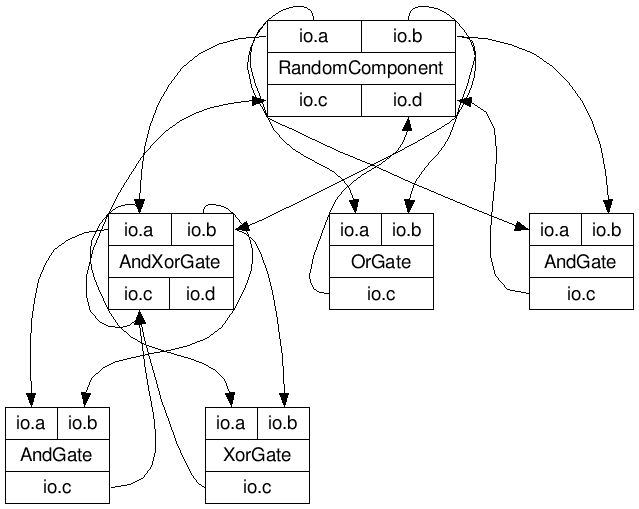
\includegraphics[width=0.7\textwidth]{img/HierarchicalLayoutSimple}
  }
  \caption[Simple hierarchical layout for diagram visualization]{The simplest
    hierarchical visualization, where parents are just represented using various
    heights}
  \label{fig:hierarchical-layout-simple}
\end{figure}

The problem by using such a representation is clearly visible, sometimes the
ports of a component is an output type port as well as an input type port.
This can be seen at the port "io.c" from the \texttt{AndXorGate} component. In
listing \ref{lst:andxorgate-problem}, we can see that the value \verb|io.c| is
written as an output of the component. In the figure
\ref{fig:hierarchical-layout-simple}, the same port is the source and the target
of some connections. This can cause some misunderstanding.

\begin{listing}[H]
  \centering
\begin{scalacode}
class AndXorGate extends Component {

  val xorGate = new XorGate
  val andGate = new AndGate

  val io = new Bundle {
    val a: Bool = in Bool
    val b: Bool = in Bool
    val c: Bool = out Bool
    val d: Bool = out Bool
  }

  xorGate.io.a := io.a
  xorGate.io.b := io.b
  andGate.io.a := io.a
  andGate.io.b := io.b

  io.c := xorGate.io.c
  io.d := andGate.io.c
}
\end{scalacode}
  \caption[The AndXorGate component written with SpinalHDL]{The AndXorGate
component written with SpinalHDL. We can see that the ``c'' port is an output
of the components and in figure \ref{fig:hierarchical-layout-simple} the port is
shown as an input port and as an output port.}
  \label{lst:andxorgate-problem}
\end{listing}

\subsection{Tree view}

The idea of the tree view is to represent the hierarchical relation like in file
explorer. The figure \ref{fig:tree-view} depicts the idea for a SpinalHDL
component.

\begin{figure}[H]
  \centering
  \fbox{
    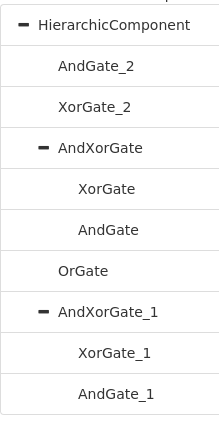
\includegraphics[width=0.2\textwidth]{img/tree-view}
  }
  \caption[SpinalHDL's Component visualization with tree view]{A tree view
    visualization of a SpinalHDL component, each child is under its parent and
    eventually possesses itself some sub-components.}
  \label{fig:tree-view}
\end{figure}

The tree view visualization is very useful to directly detect the relation
between some components. The big problem is that we can't see the connection
relationships.

\subsection{Multiple diagrams}

As seen with the hierarchical layout figure
\ref{fig:hierarchical-layout-simple}, the problem is that sometimes a port is an
output for some components and, in the other way, an input for some other
ones. If we look closely to the problem we could notice that a port receives
connections from its brothers and sends connections to its childrens.

\begin{figure}[H]
  \centering
  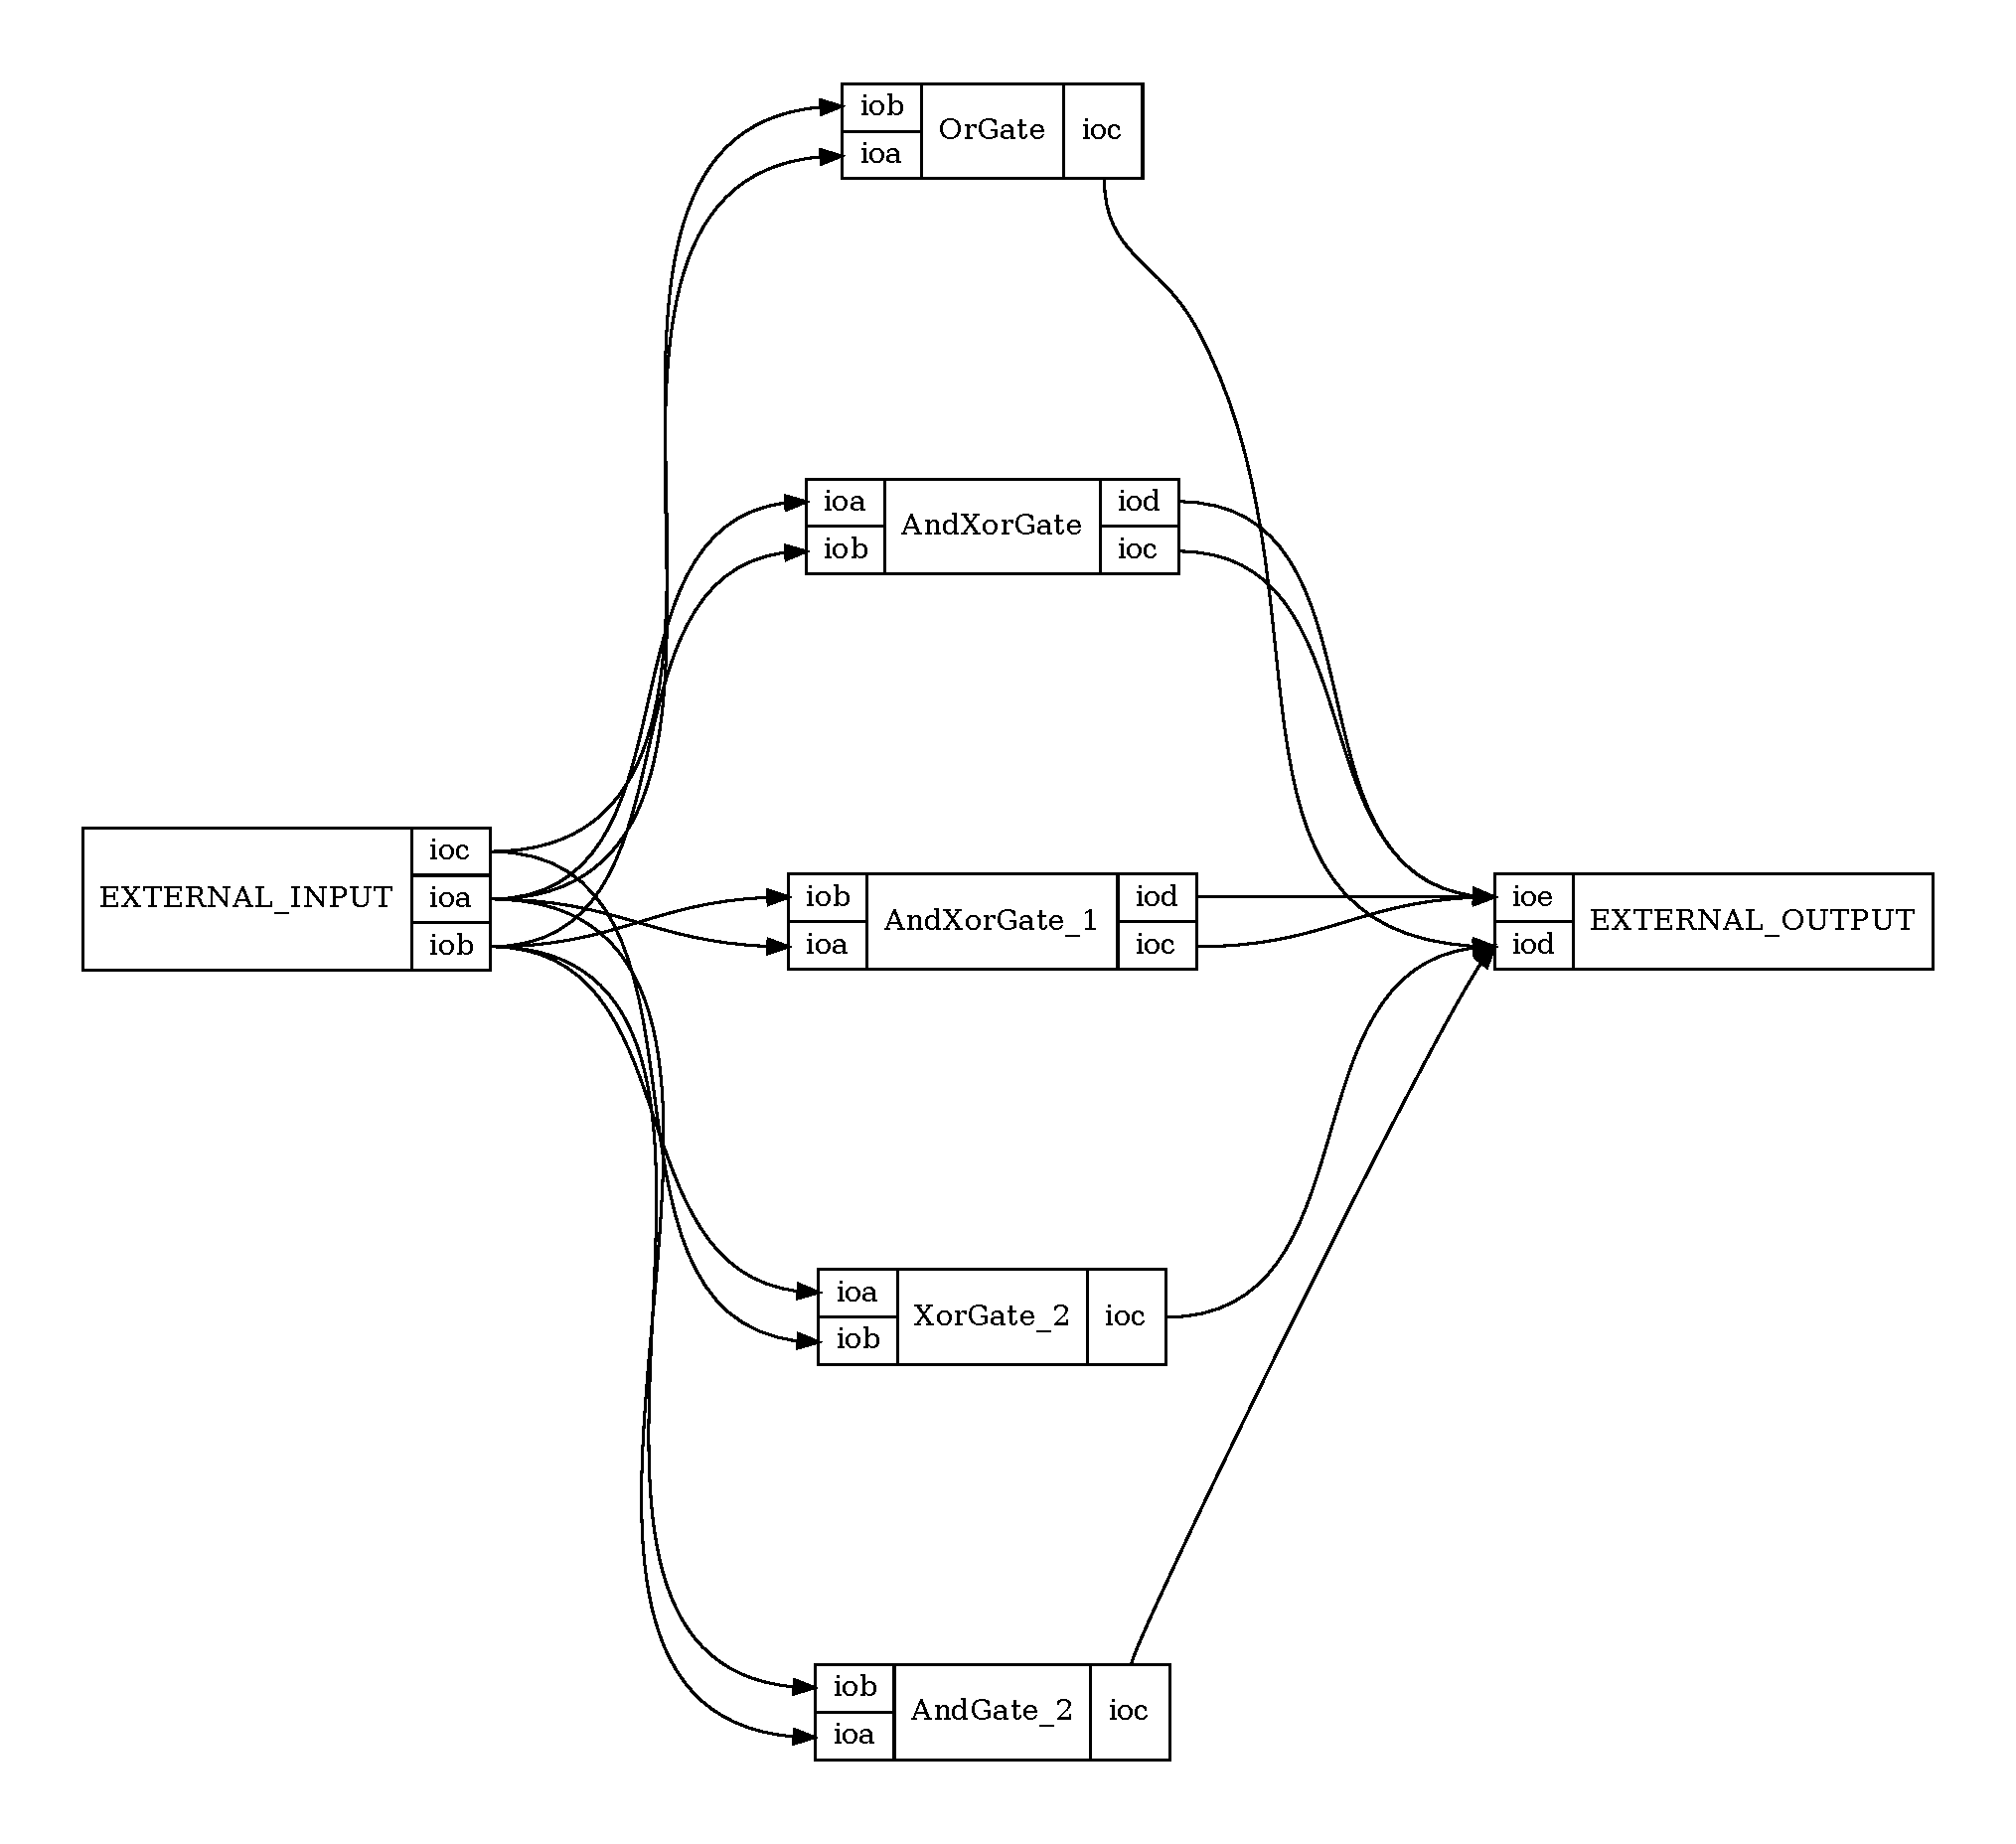
\includegraphics[width=0.6\textwidth]{img/HierarchicComponent.pdf}
  \caption[SpinalHDL Component inside]{Inside a SpinalHDL component, the
    component owns inputs and outputs on his own interface and communicates
  with its children}
  \label{fig:hierarchic-component}
\end{figure}

\begin{figure}[H]
  \centering
  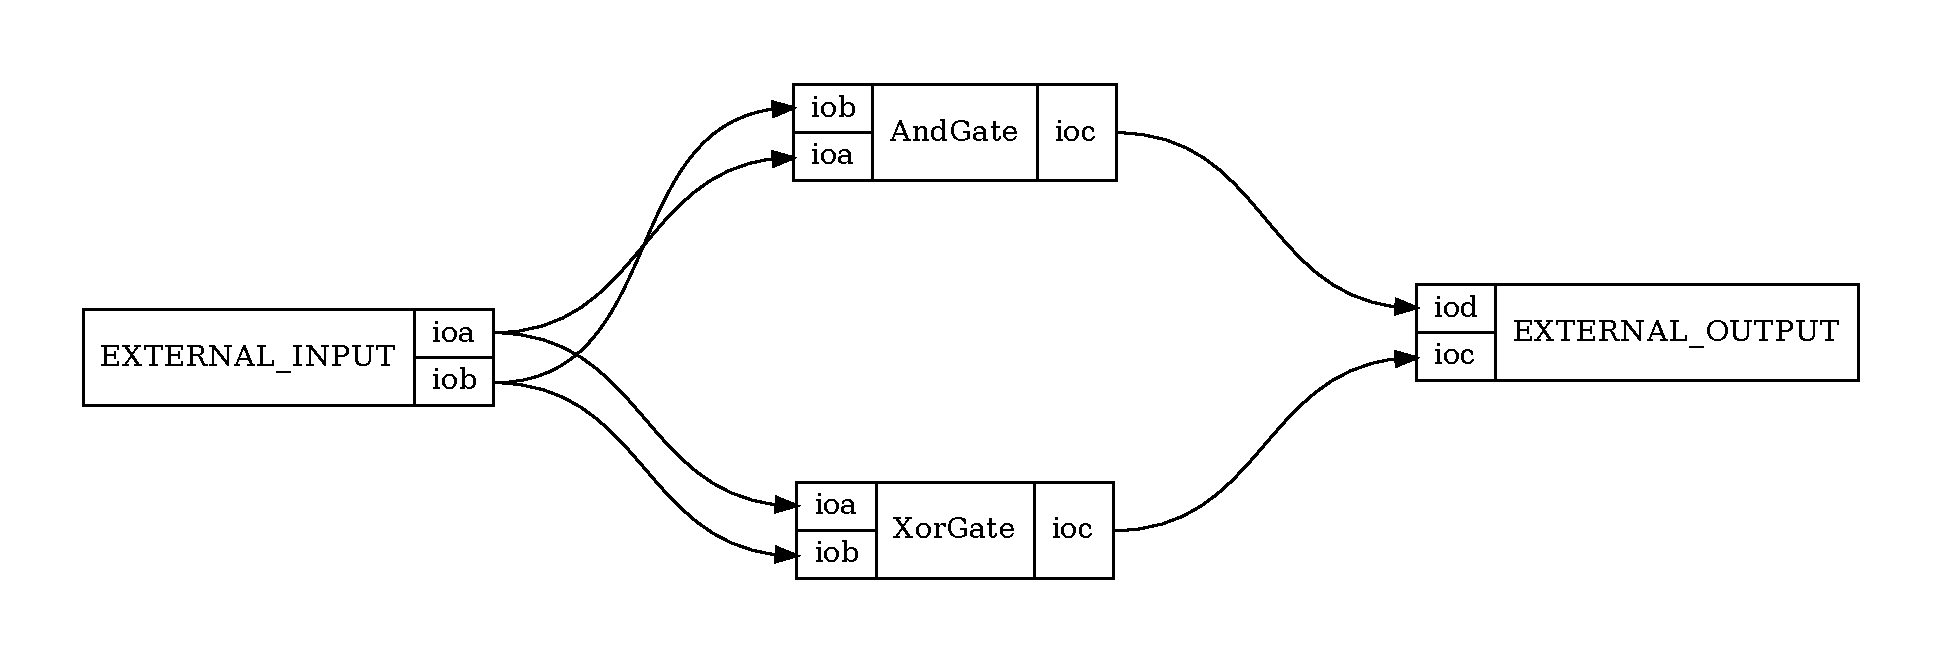
\includegraphics[width=0.6\textwidth]{img/AndXorGate.pdf}
  \caption[SpinalHDL Component inside an another]{Component which is the
    sub-component of the component from figure \ref{fig:hierarchic-component},
    the external inputs and outputs are corresponding to the ones in the parent component}
  \label{fig:and-xor-gate}
\end{figure}

Using such a representation solves the problem discussed in
\ref{sec:hierarchical-layout} : if we represent all the components just using
one diagram, sometimes the ports are inputs and sometimes they are outputs. With
multiple diagrams this problem does not occur anymore.

The major disadvantage is that we need an interactive diagram for exploring
the children of a component or multiple static ones which is not practical.

\section{A visual example}

The diagram we want to produce, as explained in chapter \ref{sec:graph-layout}, owns the following properties :
\begin{itemize}
  \item Oriented
  \item Cyclic
  \item Connection between ports on nodes and not between nodes
\end{itemize}

\section{Model representation}
\label{sec:model-representation} 

The model representation is buildt using the object-oriented paradigm. The
figure \ref{fig:model-class-diagram} shows the class diagram of the models.

\begin{figure}[H]
  \centering
  \fbox{
  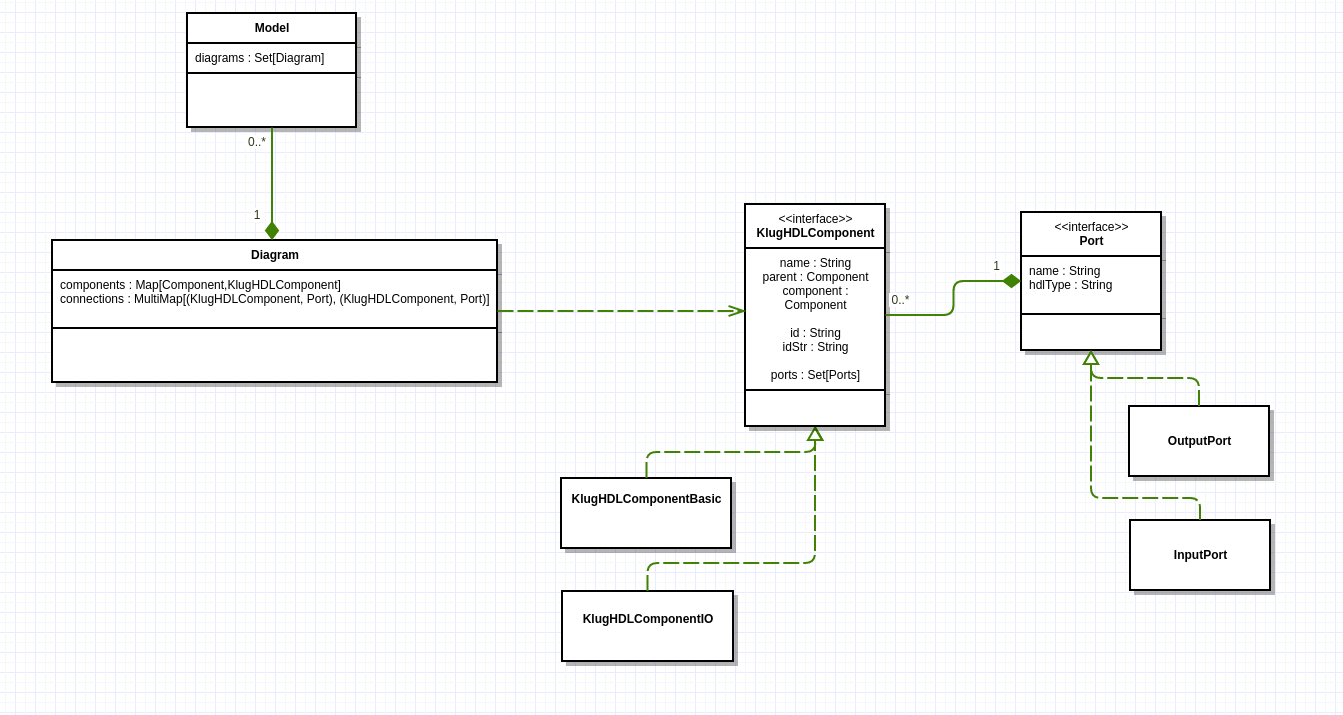
\includegraphics[width=0.99\textwidth]{img/class-diagram-intermeditate-model}
  }
  \caption[Class diagram of the intermediate model]{The complete class diagram of the intermediate model representation}
  \label{fig:model-class-diagram}
\end{figure}

\section{Conclusion}

The major advantage of such an intermediate representation is the capability to
evolve the program in order to produce additional outputs. For now there is just
a \textbf{DOT} and \textbf{JSON} backend. It also provides a way to check the
correctness of the diagram after the parsing on the AST : connections with
non-existing port for example.

%%% Local Variables:
%%% mode: latex
%%% TeX-master: "../report"
%%% End:
